% Created by tikzDevice version 0.12.3.1 on 2023-06-16 17:16:15
% !TEX encoding = UTF-8 Unicode
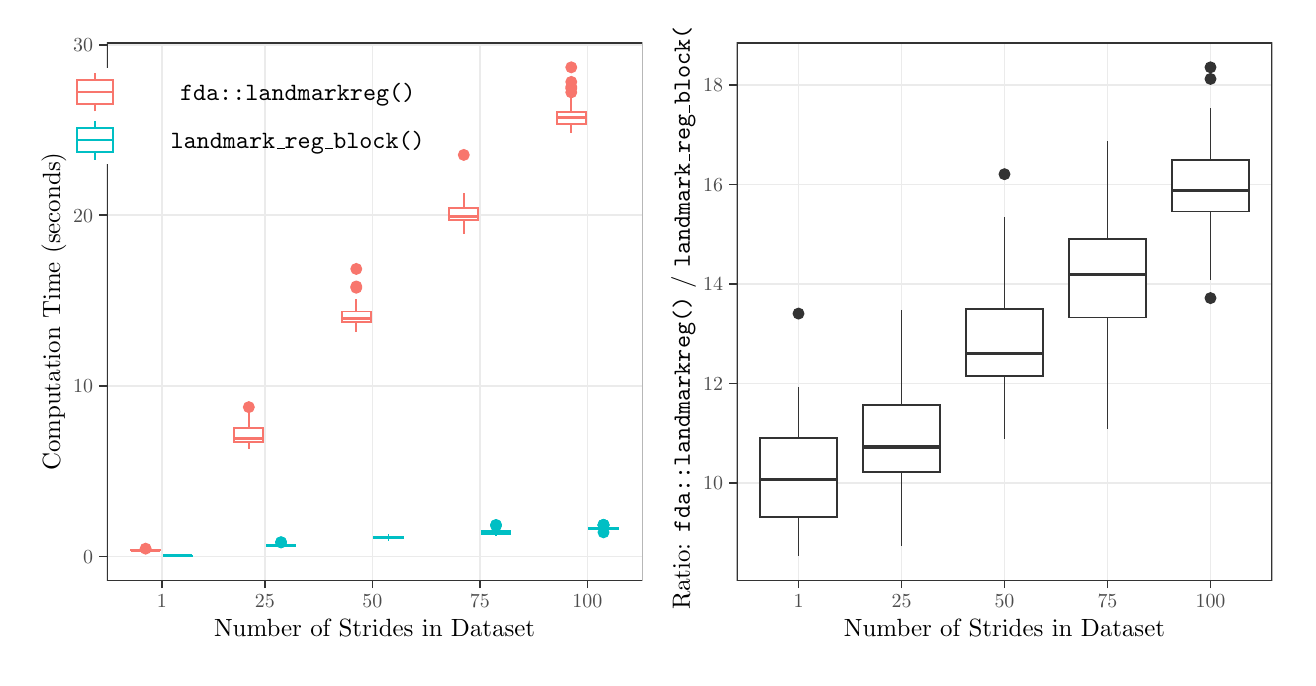
\begin{tikzpicture}[x=1pt,y=1pt]
\definecolor{fillColor}{RGB}{255,255,255}
\path[use as bounding box,fill=fillColor,fill opacity=0.00] (0,0) rectangle (455.24,227.62);
\begin{scope}
\path[clip] (  0.00,  0.00) rectangle (227.62,227.62);
\definecolor{drawColor}{RGB}{255,255,255}
\definecolor{fillColor}{RGB}{255,255,255}

\path[draw=drawColor,line width= 0.6pt,line join=round,line cap=round,fill=fillColor] ( -0.00,  0.00) rectangle (227.62,227.62);
\end{scope}
\begin{scope}
\path[clip] ( 28.58, 27.89) rectangle (222.12,222.12);
\definecolor{fillColor}{RGB}{255,255,255}

\path[fill=fillColor] ( 28.58, 27.89) rectangle (222.12,222.12);
\definecolor{drawColor}{gray}{0.92}

\path[draw=drawColor,line width= 0.6pt,line join=round] ( 28.58, 36.55) --
	(222.12, 36.55);

\path[draw=drawColor,line width= 0.6pt,line join=round] ( 28.58, 98.19) --
	(222.12, 98.19);

\path[draw=drawColor,line width= 0.6pt,line join=round] ( 28.58,159.82) --
	(222.12,159.82);

\path[draw=drawColor,line width= 0.6pt,line join=round] ( 28.58,221.45) --
	(222.12,221.45);

\path[draw=drawColor,line width= 0.6pt,line join=round] ( 48.45, 27.89) --
	( 48.45,222.12);

\path[draw=drawColor,line width= 0.6pt,line join=round] ( 85.74, 27.89) --
	( 85.74,222.12);

\path[draw=drawColor,line width= 0.6pt,line join=round] (124.58, 27.89) --
	(124.58,222.12);

\path[draw=drawColor,line width= 0.6pt,line join=round] (163.42, 27.89) --
	(163.42,222.12);

\path[draw=drawColor,line width= 0.6pt,line join=round] (202.26, 27.89) --
	(202.26,222.12);
\definecolor{drawColor}{RGB}{248,118,109}
\definecolor{fillColor}{RGB}{248,118,109}

\path[draw=drawColor,line width= 0.4pt,line join=round,line cap=round,fill=fillColor] ( 42.62, 39.36) circle (  1.96);

\path[draw=drawColor,line width= 0.6pt,line join=round] ( 42.62, 38.83) -- ( 42.62, 38.92);

\path[draw=drawColor,line width= 0.6pt,line join=round] ( 42.62, 38.76) -- ( 42.62, 38.66);
\definecolor{fillColor}{RGB}{255,255,255}

\path[draw=drawColor,line width= 0.6pt,fill=fillColor] ( 37.38, 38.83) --
	( 37.38, 38.76) --
	( 47.87, 38.76) --
	( 47.87, 38.83) --
	( 37.38, 38.83) --
	cycle;

\path[draw=drawColor,line width= 1.1pt] ( 37.38, 38.81) -- ( 47.87, 38.81);
\definecolor{fillColor}{RGB}{248,118,109}

\path[draw=drawColor,line width= 0.4pt,line join=round,line cap=round,fill=fillColor] ( 79.91, 90.50) circle (  1.96);

\path[draw=drawColor,line width= 0.6pt,line join=round] ( 79.91, 82.96) -- ( 79.91, 89.70);

\path[draw=drawColor,line width= 0.6pt,line join=round] ( 79.91, 77.93) -- ( 79.91, 75.52);
\definecolor{fillColor}{RGB}{255,255,255}

\path[draw=drawColor,line width= 0.6pt,fill=fillColor] ( 74.67, 82.96) --
	( 74.67, 77.93) --
	( 85.15, 77.93) --
	( 85.15, 82.96) --
	( 74.67, 82.96) --
	cycle;

\path[draw=drawColor,line width= 1.1pt] ( 74.67, 79.26) -- ( 85.15, 79.26);
\definecolor{fillColor}{RGB}{248,118,109}

\path[draw=drawColor,line width= 0.4pt,line join=round,line cap=round,fill=fillColor] (118.75,133.64) circle (  1.96);

\path[draw=drawColor,line width= 0.4pt,line join=round,line cap=round,fill=fillColor] (118.75,134.11) circle (  1.96);

\path[draw=drawColor,line width= 0.4pt,line join=round,line cap=round,fill=fillColor] (118.75,140.44) circle (  1.96);

\path[draw=drawColor,line width= 0.6pt,line join=round] (118.75,125.08) -- (118.75,129.47);

\path[draw=drawColor,line width= 0.6pt,line join=round] (118.75,121.33) -- (118.75,117.79);
\definecolor{fillColor}{RGB}{255,255,255}

\path[draw=drawColor,line width= 0.6pt,fill=fillColor] (113.51,125.08) --
	(113.51,121.33) --
	(123.99,121.33) --
	(123.99,125.08) --
	(113.51,125.08) --
	cycle;

\path[draw=drawColor,line width= 1.1pt] (113.51,122.60) -- (123.99,122.60);
\definecolor{fillColor}{RGB}{248,118,109}

\path[draw=drawColor,line width= 0.4pt,line join=round,line cap=round,fill=fillColor] (157.59,181.64) circle (  1.96);

\path[draw=drawColor,line width= 0.6pt,line join=round] (157.59,162.57) -- (157.59,168.05);

\path[draw=drawColor,line width= 0.6pt,line join=round] (157.59,158.12) -- (157.59,153.07);
\definecolor{fillColor}{RGB}{255,255,255}

\path[draw=drawColor,line width= 0.6pt,fill=fillColor] (152.35,162.57) --
	(152.35,158.12) --
	(162.83,158.12) --
	(162.83,162.57) --
	(152.35,162.57) --
	cycle;

\path[draw=drawColor,line width= 1.1pt] (152.35,159.40) -- (162.83,159.40);
\definecolor{fillColor}{RGB}{248,118,109}

\path[draw=drawColor,line width= 0.4pt,line join=round,line cap=round,fill=fillColor] (196.43,208.02) circle (  1.96);

\path[draw=drawColor,line width= 0.4pt,line join=round,line cap=round,fill=fillColor] (196.43,213.29) circle (  1.96);

\path[draw=drawColor,line width= 0.4pt,line join=round,line cap=round,fill=fillColor] (196.43,206.21) circle (  1.96);

\path[draw=drawColor,line width= 0.4pt,line join=round,line cap=round,fill=fillColor] (196.43,205.66) circle (  1.96);

\path[draw=drawColor,line width= 0.4pt,line join=round,line cap=round,fill=fillColor] (196.43,204.25) circle (  1.96);

\path[draw=drawColor,line width= 0.6pt,line join=round] (196.43,197.18) -- (196.43,202.88);

\path[draw=drawColor,line width= 0.6pt,line join=round] (196.43,192.70) -- (196.43,189.41);
\definecolor{fillColor}{RGB}{255,255,255}

\path[draw=drawColor,line width= 0.6pt,fill=fillColor] (191.19,197.18) --
	(191.19,192.70) --
	(201.67,192.70) --
	(201.67,197.18) --
	(191.19,197.18) --
	cycle;

\path[draw=drawColor,line width= 1.1pt] (191.19,195.25) -- (201.67,195.25);
\definecolor{drawColor}{RGB}{0,191,196}

\path[draw=drawColor,line width= 0.6pt,line join=round] ( 54.28, 36.79) -- ( 54.28, 36.81);

\path[draw=drawColor,line width= 0.6pt,line join=round] ( 54.28, 36.76) -- ( 54.28, 36.72);

\path[draw=drawColor,line width= 0.6pt,fill=fillColor] ( 49.03, 36.79) --
	( 49.03, 36.76) --
	( 59.52, 36.76) --
	( 59.52, 36.79) --
	( 49.03, 36.79) --
	cycle;

\path[draw=drawColor,line width= 1.1pt] ( 49.03, 36.78) -- ( 59.52, 36.78);
\definecolor{fillColor}{RGB}{0,191,196}

\path[draw=drawColor,line width= 0.4pt,line join=round,line cap=round,fill=fillColor] ( 91.56, 41.64) circle (  1.96);

\path[draw=drawColor,line width= 0.4pt,line join=round,line cap=round,fill=fillColor] ( 91.56, 41.68) circle (  1.96);

\path[draw=drawColor,line width= 0.6pt,line join=round] ( 91.56, 40.81) -- ( 91.56, 41.46);

\path[draw=drawColor,line width= 0.6pt,line join=round] ( 91.56, 40.35) -- ( 91.56, 39.84);
\definecolor{fillColor}{RGB}{255,255,255}

\path[draw=drawColor,line width= 0.6pt,fill=fillColor] ( 86.32, 40.81) --
	( 86.32, 40.35) --
	( 96.81, 40.35) --
	( 96.81, 40.81) --
	( 86.32, 40.81) --
	cycle;

\path[draw=drawColor,line width= 1.1pt] ( 86.32, 40.54) -- ( 96.81, 40.54);

\path[draw=drawColor,line width= 0.6pt,line join=round] (130.40, 43.66) -- (130.40, 44.58);

\path[draw=drawColor,line width= 0.6pt,line join=round] (130.40, 42.98) -- (130.40, 42.09);

\path[draw=drawColor,line width= 0.6pt,fill=fillColor] (125.16, 43.66) --
	(125.16, 42.98) --
	(135.65, 42.98) --
	(135.65, 43.66) --
	(125.16, 43.66) --
	cycle;

\path[draw=drawColor,line width= 1.1pt] (125.16, 43.29) -- (135.65, 43.29);
\definecolor{fillColor}{RGB}{0,191,196}

\path[draw=drawColor,line width= 0.4pt,line join=round,line cap=round,fill=fillColor] (169.24, 47.73) circle (  1.96);

\path[draw=drawColor,line width= 0.4pt,line join=round,line cap=round,fill=fillColor] (169.24, 47.93) circle (  1.96);

\path[draw=drawColor,line width= 0.6pt,line join=round] (169.24, 45.68) -- (169.24, 46.99);

\path[draw=drawColor,line width= 0.6pt,line join=round] (169.24, 44.75) -- (169.24, 44.04);
\definecolor{fillColor}{RGB}{255,255,255}

\path[draw=drawColor,line width= 0.6pt,fill=fillColor] (164.00, 45.68) --
	(164.00, 44.75) --
	(174.48, 44.75) --
	(174.48, 45.68) --
	(164.00, 45.68) --
	cycle;

\path[draw=drawColor,line width= 1.1pt] (164.00, 45.25) -- (174.48, 45.25);
\definecolor{fillColor}{RGB}{0,191,196}

\path[draw=drawColor,line width= 0.4pt,line join=round,line cap=round,fill=fillColor] (208.08, 47.89) circle (  1.96);

\path[draw=drawColor,line width= 0.4pt,line join=round,line cap=round,fill=fillColor] (208.08, 47.94) circle (  1.96);

\path[draw=drawColor,line width= 0.4pt,line join=round,line cap=round,fill=fillColor] (208.08, 45.26) circle (  1.96);

\path[draw=drawColor,line width= 0.4pt,line join=round,line cap=round,fill=fillColor] (208.08, 47.94) circle (  1.96);

\path[draw=drawColor,line width= 0.4pt,line join=round,line cap=round,fill=fillColor] (208.08, 47.92) circle (  1.96);

\path[draw=drawColor,line width= 0.6pt,line join=round] (208.08, 46.82) -- (208.08, 47.50);

\path[draw=drawColor,line width= 0.6pt,line join=round] (208.08, 46.23) -- (208.08, 45.44);
\definecolor{fillColor}{RGB}{255,255,255}

\path[draw=drawColor,line width= 0.6pt,fill=fillColor] (202.84, 46.82) --
	(202.84, 46.23) --
	(213.32, 46.23) --
	(213.32, 46.82) --
	(202.84, 46.82) --
	cycle;

\path[draw=drawColor,line width= 1.1pt] (202.84, 46.56) -- (213.32, 46.56);
\definecolor{drawColor}{gray}{0.20}

\path[draw=drawColor,line width= 0.6pt,line join=round,line cap=round] ( 28.58, 27.89) rectangle (222.12,222.12);
\end{scope}
\begin{scope}
\path[clip] (  0.00,  0.00) rectangle (455.24,227.62);
\definecolor{drawColor}{gray}{0.30}

\node[text=drawColor,anchor=base east,inner sep=0pt, outer sep=0pt, scale=  0.72] at ( 23.63, 34.07) {0};

\node[text=drawColor,anchor=base east,inner sep=0pt, outer sep=0pt, scale=  0.72] at ( 23.63, 95.71) {10};

\node[text=drawColor,anchor=base east,inner sep=0pt, outer sep=0pt, scale=  0.72] at ( 23.63,157.34) {20};

\node[text=drawColor,anchor=base east,inner sep=0pt, outer sep=0pt, scale=  0.72] at ( 23.63,218.97) {30};
\end{scope}
\begin{scope}
\path[clip] (  0.00,  0.00) rectangle (455.24,227.62);
\definecolor{drawColor}{gray}{0.20}

\path[draw=drawColor,line width= 0.6pt,line join=round] ( 25.83, 36.55) --
	( 28.58, 36.55);

\path[draw=drawColor,line width= 0.6pt,line join=round] ( 25.83, 98.19) --
	( 28.58, 98.19);

\path[draw=drawColor,line width= 0.6pt,line join=round] ( 25.83,159.82) --
	( 28.58,159.82);

\path[draw=drawColor,line width= 0.6pt,line join=round] ( 25.83,221.45) --
	( 28.58,221.45);
\end{scope}
\begin{scope}
\path[clip] (  0.00,  0.00) rectangle (455.24,227.62);
\definecolor{drawColor}{gray}{0.20}

\path[draw=drawColor,line width= 0.6pt,line join=round] ( 48.45, 25.14) --
	( 48.45, 27.89);

\path[draw=drawColor,line width= 0.6pt,line join=round] ( 85.74, 25.14) --
	( 85.74, 27.89);

\path[draw=drawColor,line width= 0.6pt,line join=round] (124.58, 25.14) --
	(124.58, 27.89);

\path[draw=drawColor,line width= 0.6pt,line join=round] (163.42, 25.14) --
	(163.42, 27.89);

\path[draw=drawColor,line width= 0.6pt,line join=round] (202.26, 25.14) --
	(202.26, 27.89);
\end{scope}
\begin{scope}
\path[clip] (  0.00,  0.00) rectangle (455.24,227.62);
\definecolor{drawColor}{gray}{0.30}

\node[text=drawColor,anchor=base,inner sep=0pt, outer sep=0pt, scale=  0.72] at ( 48.45, 17.98) {1};

\node[text=drawColor,anchor=base,inner sep=0pt, outer sep=0pt, scale=  0.72] at ( 85.74, 17.98) {25};

\node[text=drawColor,anchor=base,inner sep=0pt, outer sep=0pt, scale=  0.72] at (124.58, 17.98) {50};

\node[text=drawColor,anchor=base,inner sep=0pt, outer sep=0pt, scale=  0.72] at (163.42, 17.98) {75};

\node[text=drawColor,anchor=base,inner sep=0pt, outer sep=0pt, scale=  0.72] at (202.26, 17.98) {100};
\end{scope}
\begin{scope}
\path[clip] (  0.00,  0.00) rectangle (455.24,227.62);
\definecolor{drawColor}{RGB}{0,0,0}

\node[text=drawColor,anchor=base,inner sep=0pt, outer sep=0pt, scale=  0.90] at (125.35,  7.49) {Number of Strides in Dataset};
\end{scope}
\begin{scope}
\path[clip] (  0.00,  0.00) rectangle (455.24,227.62);
\definecolor{drawColor}{RGB}{0,0,0}

\node[text=drawColor,rotate= 90.00,anchor=base,inner sep=0pt, outer sep=0pt, scale=  0.90] at ( 11.70,125.01) {Computation Time (seconds)};
\end{scope}
\begin{scope}
\path[clip] (  0.00,  0.00) rectangle (455.24,227.62);
\definecolor{fillColor}{RGB}{255,255,255}

\path[fill=fillColor] ( 15.63,195.59) rectangle ( 32.98,212.94);
\end{scope}
\begin{scope}
\path[clip] (  0.00,  0.00) rectangle (455.24,227.62);
\definecolor{drawColor}{RGB}{248,118,109}

\path[draw=drawColor,line width= 0.6pt] ( 24.30,197.33) --
	( 24.30,199.93);

\path[draw=drawColor,line width= 0.6pt] ( 24.30,208.60) --
	( 24.30,211.20);
\definecolor{fillColor}{RGB}{255,255,255}

\path[draw=drawColor,line width= 0.6pt,fill=fillColor] ( 17.80,199.93) rectangle ( 30.81,208.60);

\path[draw=drawColor,line width= 0.6pt] ( 17.80,204.27) --
	( 30.81,204.27);
\end{scope}
\begin{scope}
\path[clip] (  0.00,  0.00) rectangle (455.24,227.62);
\definecolor{fillColor}{RGB}{255,255,255}

\path[fill=fillColor] ( 15.63,178.25) rectangle ( 32.98,195.59);
\end{scope}
\begin{scope}
\path[clip] (  0.00,  0.00) rectangle (455.24,227.62);
\definecolor{drawColor}{RGB}{0,191,196}

\path[draw=drawColor,line width= 0.6pt] ( 24.30,179.98) --
	( 24.30,182.58);

\path[draw=drawColor,line width= 0.6pt] ( 24.30,191.26) --
	( 24.30,193.86);
\definecolor{fillColor}{RGB}{255,255,255}

\path[draw=drawColor,line width= 0.6pt,fill=fillColor] ( 17.80,182.58) rectangle ( 30.81,191.26);

\path[draw=drawColor,line width= 0.6pt] ( 17.80,186.92) --
	( 30.81,186.92);
\end{scope}
\begin{scope}
\path[clip] (  0.00,  0.00) rectangle (455.24,227.62);
\definecolor{drawColor}{RGB}{0,0,0}

\node[text=drawColor,anchor=base,inner sep=0pt, outer sep=0pt, scale=  0.90] at ( 97.57,201.17) {\texttt{fda::landmarkreg()}};
\end{scope}
\begin{scope}
\path[clip] (  0.00,  0.00) rectangle (455.24,227.62);
\definecolor{drawColor}{RGB}{0,0,0}

\node[text=drawColor,anchor=base,inner sep=0pt, outer sep=0pt, scale=  0.90] at ( 97.57,183.82) {\texttt{landmark\_reg\_block()}};
\end{scope}
\begin{scope}
\path[clip] (227.62,  0.00) rectangle (455.24,227.62);
\definecolor{drawColor}{RGB}{255,255,255}
\definecolor{fillColor}{RGB}{255,255,255}

\path[draw=drawColor,line width= 0.6pt,line join=round,line cap=round,fill=fillColor] (227.62,  0.00) rectangle (455.24,227.62);
\end{scope}
\begin{scope}
\path[clip] (256.21, 27.89) rectangle (449.74,222.12);
\definecolor{fillColor}{RGB}{255,255,255}

\path[fill=fillColor] (256.21, 27.89) rectangle (449.74,222.12);
\definecolor{drawColor}{gray}{0.92}

\path[draw=drawColor,line width= 0.6pt,line join=round] (256.21, 63.04) --
	(449.74, 63.04);

\path[draw=drawColor,line width= 0.6pt,line join=round] (256.21, 99.00) --
	(449.74, 99.00);

\path[draw=drawColor,line width= 0.6pt,line join=round] (256.21,134.97) --
	(449.74,134.97);

\path[draw=drawColor,line width= 0.6pt,line join=round] (256.21,170.94) --
	(449.74,170.94);

\path[draw=drawColor,line width= 0.6pt,line join=round] (256.21,206.90) --
	(449.74,206.90);

\path[draw=drawColor,line width= 0.6pt,line join=round] (278.54, 27.89) --
	(278.54,222.12);

\path[draw=drawColor,line width= 0.6pt,line join=round] (315.76, 27.89) --
	(315.76,222.12);

\path[draw=drawColor,line width= 0.6pt,line join=round] (352.97, 27.89) --
	(352.97,222.12);

\path[draw=drawColor,line width= 0.6pt,line join=round] (390.19, 27.89) --
	(390.19,222.12);

\path[draw=drawColor,line width= 0.6pt,line join=round] (427.41, 27.89) --
	(427.41,222.12);
\definecolor{drawColor}{gray}{0.20}
\definecolor{fillColor}{gray}{0.20}

\path[draw=drawColor,line width= 0.4pt,line join=round,line cap=round,fill=fillColor] (278.54,124.31) circle (  1.96);

\path[draw=drawColor,line width= 0.6pt,line join=round] (278.54, 79.42) -- (278.54, 97.84);

\path[draw=drawColor,line width= 0.6pt,line join=round] (278.54, 50.89) -- (278.54, 36.72);
\definecolor{fillColor}{RGB}{255,255,255}

\path[draw=drawColor,line width= 0.6pt,fill=fillColor] (264.58, 79.42) --
	(264.58, 50.89) --
	(292.49, 50.89) --
	(292.49, 79.42) --
	(264.58, 79.42) --
	cycle;

\path[draw=drawColor,line width= 1.1pt] (264.58, 64.34) -- (292.49, 64.34);

\path[draw=drawColor,line width= 0.6pt,line join=round] (315.76, 91.25) -- (315.76,125.68);

\path[draw=drawColor,line width= 0.6pt,line join=round] (315.76, 66.99) -- (315.76, 40.37);

\path[draw=drawColor,line width= 0.6pt,fill=fillColor] (301.80, 91.25) --
	(301.80, 66.99) --
	(329.71, 66.99) --
	(329.71, 91.25) --
	(301.80, 91.25) --
	cycle;

\path[draw=drawColor,line width= 1.1pt] (301.80, 76.09) -- (329.71, 76.09);
\definecolor{fillColor}{gray}{0.20}

\path[draw=drawColor,line width= 0.4pt,line join=round,line cap=round,fill=fillColor] (352.97,174.68) circle (  1.96);

\path[draw=drawColor,line width= 0.6pt,line join=round] (352.97,125.99) -- (352.97,159.26);

\path[draw=drawColor,line width= 0.6pt,line join=round] (352.97,101.68) -- (352.97, 79.09);
\definecolor{fillColor}{RGB}{255,255,255}

\path[draw=drawColor,line width= 0.6pt,fill=fillColor] (339.02,125.99) --
	(339.02,101.68) --
	(366.93,101.68) --
	(366.93,125.99) --
	(339.02,125.99) --
	cycle;

\path[draw=drawColor,line width= 1.1pt] (339.02,109.78) -- (366.93,109.78);

\path[draw=drawColor,line width= 0.6pt,line join=round] (390.19,151.21) -- (390.19,186.80);

\path[draw=drawColor,line width= 0.6pt,line join=round] (390.19,122.86) -- (390.19, 82.47);

\path[draw=drawColor,line width= 0.6pt,fill=fillColor] (376.24,151.21) --
	(376.24,122.86) --
	(404.15,122.86) --
	(404.15,151.21) --
	(376.24,151.21) --
	cycle;

\path[draw=drawColor,line width= 1.1pt] (376.24,138.45) -- (404.15,138.45);
\definecolor{fillColor}{gray}{0.20}

\path[draw=drawColor,line width= 0.4pt,line join=round,line cap=round,fill=fillColor] (427.41,209.10) circle (  1.96);

\path[draw=drawColor,line width= 0.4pt,line join=round,line cap=round,fill=fillColor] (427.41,213.29) circle (  1.96);

\path[draw=drawColor,line width= 0.4pt,line join=round,line cap=round,fill=fillColor] (427.41,129.90) circle (  1.96);

\path[draw=drawColor,line width= 0.6pt,line join=round] (427.41,179.74) -- (427.41,198.68);

\path[draw=drawColor,line width= 0.6pt,line join=round] (427.41,161.15) -- (427.41,136.44);
\definecolor{fillColor}{RGB}{255,255,255}

\path[draw=drawColor,line width= 0.6pt,fill=fillColor] (413.45,179.74) --
	(413.45,161.15) --
	(441.37,161.15) --
	(441.37,179.74) --
	(413.45,179.74) --
	cycle;

\path[draw=drawColor,line width= 1.1pt] (413.45,168.89) -- (441.37,168.89);

\path[draw=drawColor,line width= 0.6pt,line join=round,line cap=round] (256.21, 27.89) rectangle (449.74,222.12);
\end{scope}
\begin{scope}
\path[clip] (  0.00,  0.00) rectangle (455.24,227.62);
\definecolor{drawColor}{gray}{0.30}

\node[text=drawColor,anchor=base east,inner sep=0pt, outer sep=0pt, scale=  0.72] at (251.26, 60.56) {10};

\node[text=drawColor,anchor=base east,inner sep=0pt, outer sep=0pt, scale=  0.72] at (251.26, 96.52) {12};

\node[text=drawColor,anchor=base east,inner sep=0pt, outer sep=0pt, scale=  0.72] at (251.26,132.49) {14};

\node[text=drawColor,anchor=base east,inner sep=0pt, outer sep=0pt, scale=  0.72] at (251.26,168.46) {16};

\node[text=drawColor,anchor=base east,inner sep=0pt, outer sep=0pt, scale=  0.72] at (251.26,204.42) {18};
\end{scope}
\begin{scope}
\path[clip] (  0.00,  0.00) rectangle (455.24,227.62);
\definecolor{drawColor}{gray}{0.20}

\path[draw=drawColor,line width= 0.6pt,line join=round] (253.46, 63.04) --
	(256.21, 63.04);

\path[draw=drawColor,line width= 0.6pt,line join=round] (253.46, 99.00) --
	(256.21, 99.00);

\path[draw=drawColor,line width= 0.6pt,line join=round] (253.46,134.97) --
	(256.21,134.97);

\path[draw=drawColor,line width= 0.6pt,line join=round] (253.46,170.94) --
	(256.21,170.94);

\path[draw=drawColor,line width= 0.6pt,line join=round] (253.46,206.90) --
	(256.21,206.90);
\end{scope}
\begin{scope}
\path[clip] (  0.00,  0.00) rectangle (455.24,227.62);
\definecolor{drawColor}{gray}{0.20}

\path[draw=drawColor,line width= 0.6pt,line join=round] (278.54, 25.14) --
	(278.54, 27.89);

\path[draw=drawColor,line width= 0.6pt,line join=round] (315.76, 25.14) --
	(315.76, 27.89);

\path[draw=drawColor,line width= 0.6pt,line join=round] (352.97, 25.14) --
	(352.97, 27.89);

\path[draw=drawColor,line width= 0.6pt,line join=round] (390.19, 25.14) --
	(390.19, 27.89);

\path[draw=drawColor,line width= 0.6pt,line join=round] (427.41, 25.14) --
	(427.41, 27.89);
\end{scope}
\begin{scope}
\path[clip] (  0.00,  0.00) rectangle (455.24,227.62);
\definecolor{drawColor}{gray}{0.30}

\node[text=drawColor,anchor=base,inner sep=0pt, outer sep=0pt, scale=  0.72] at (278.54, 17.98) {1};

\node[text=drawColor,anchor=base,inner sep=0pt, outer sep=0pt, scale=  0.72] at (315.76, 17.98) {25};

\node[text=drawColor,anchor=base,inner sep=0pt, outer sep=0pt, scale=  0.72] at (352.97, 17.98) {50};

\node[text=drawColor,anchor=base,inner sep=0pt, outer sep=0pt, scale=  0.72] at (390.19, 17.98) {75};

\node[text=drawColor,anchor=base,inner sep=0pt, outer sep=0pt, scale=  0.72] at (427.41, 17.98) {100};
\end{scope}
\begin{scope}
\path[clip] (  0.00,  0.00) rectangle (455.24,227.62);
\definecolor{drawColor}{RGB}{0,0,0}

\node[text=drawColor,anchor=base,inner sep=0pt, outer sep=0pt, scale=  0.90] at (352.97,  7.49) {Number of Strides in Dataset};
\end{scope}
\begin{scope}
\path[clip] (  0.00,  0.00) rectangle (455.24,227.62);
\definecolor{drawColor}{RGB}{0,0,0}

\node[text=drawColor,rotate= 90.00,anchor=base,inner sep=0pt, outer sep=0pt, scale=  0.90] at (239.32,125.01) {Ratio: \texttt{fda::landmarkreg()} / \texttt{landmark\_reg\_block()}};
\end{scope}
\end{tikzpicture}
